\documentclass[12pt, letterpaper]{article}
\usepackage{graphicx}
\usepackage[ngerman]{babel}
\usepackage{hyperref}
\usepackage{vhistory}
\usepackage{longtable}

\graphicspath{{./img/}}

\title{Technische Dokumentation}
\author{Max Riedel \and Tony Nutzmann \and Mathias Enderlein}

\begin{document}
    \begin{titlepage}
        \clearpage
        \begin{center}
        {\Large Technische Dokumentation}\\[3mm]
        {\Huge Jinba}\\[20mm]

        {vorgelegt von}\\[2mm]
        {\large Max Riedel}\\[2mm]
        {\large Tony Nutzmann}\\[2mm]
        {\large Mathias Enderlein}\\[50mm]

        
\includegraphics[width=75mm]{img/Technische_Hochschule_Brandenburg_Logo.svg.png}\\[10mm]

        {Technische Hochschule Brandenburg}\\[2mm]

        {Fachbereich Informatik}\\[2mm]

        {Studiengang Informatik}\\[20mm]

        {Betreuer \\[2mm] Ilonka Wolpert M.Sc.}
        \end{center}

        \thispagestyle{empty}
    \end{titlepage}

    \begin{versionhistory}
        \vhEntry{0.1}{28.6.2023}{Max Riedel}{Erstellung}
    \end{versionhistory}
    \newpage
    \tableofcontents
    \newpage
    \section{Einführung}

    Das Projekt Jinba, ist eine Jobplattform, die es Jobsuchenden und Unternehmen
    erleichtern soll zusammen zu finden und eine erste Kommunikationsaufnahme zu erreichen.
    Um das zu erreichen, soll die Vermittlung vorranig über die Fähigkeiten (Skills) der Jobsuchenden
    und gefordereten Fähigkeiten in den Jobangeboten eines Unternehmens erfolgen.

    Dabei ist wichtig anzumerken, dass die Plattform keinen kompletten Bewerbungsprozess
    abbilden soll, sondern nur die erste Kontaktaufnahme zwischen Unternehmen und Jobsuchenden.

    \newpage
    \section{Anwendungsfälle}
    

    \subsection{Aktoren}

    \begin{table}[htbp]
        \label{tab:aktoren}
        \begin{tabular}{|p{.25\textwidth}|p{.70\textwidth}|}
            \hline
            \textbf{Aktor} & \textbf{Beschreibung} \\
            \hline
            \hline
            Jobsuchender & Ein Jobsuchender ist eine Person, die auf der Suche nach einem Job ist. \\
            \hline
            Unternehmen & Ein Unternehmen ist eine Organisation, die Jobs anbietet. \\
            \hline
        \end{tabular}
        \caption{Liste der Aktoren}
    \end{table}

    \subsection{Anwendungsfälle}

    \begin{longtable}[htbp]{|p{.20\textwidth}|p{.20\textwidth}|p{.40\textwidth}|p{.10\textwidth}|}
       
        \hline
        \textbf{Usecase}&\textbf{Aktor}&\textbf{Beschreibung}&\textbf{Done}\\
        \hline
        \hline
        \endfirsthead

        \hline
        \textbf{Usecase}&\textbf{Aktor}&\textbf{Beschreibung}&\textbf{Done}\\
        \hline
        \hline
        \endhead

        \hline
        \endfoot

        \hline
        \caption{Anwendungsfälle}  \label{tab:Anwendungsfaelle} 
        \endlastfoot
        Registrierung& Jobsuchender, Unternehmen & Ein Benutzer kann sich auf der Plattform registrieren. & Ja \\
        \hline
        Anmeldung& Jobsuchender, Unternehmen & Ein Benutzer kann sich auf der Plattform anmelden. & Ja \\
        \hline
        Profil bearbeiten& Jobsuchender, Unternehmen & Ein Benutzer kann sein Profil bearbeiten. & Ja \\
        \hline
        Profil anzeigen& Jobsuchender, Unternehmen & Ein Benutzer kann sein Profil anzeigen. & Ja \\
        \hline
        Nach Jobs suchen& Jobsuchender & Ein Jobsuchender kann nach Jobs suchen. & Ja \\
        \hline
        Jobs vorgeschlagen bekommen& Jobsuchender & Ein Jobsuchender kann Jobs vorgeschlagen bekommen. & Ja \\
        \hline
        Jobangebot erstellen& Unternehmen & Ein Unternehmen kann ein Jobangebot erstellen. & Ja \\
        \hline
        Jobangebot bearbeiten& Unternehmen & Ein Unternehmen kann ein Jobangebot bearbeiten. & Ja \\
        \hline
        Jobangebot anzeigen& Jobsuchender, Unternehmen & Ein Benutzer kann ein Jobangebot anzeigen. & Ja \\
        \hline
        Bewerben& Jobsuchender & Ein Jobsuchender kann sich auf ein Jobangebot bewerben. & Ja \\
        \hline
        Bewerbung ansehen& Unternehmen & Ein Unternehmen kann sich die Bewerbungen auf ein Jobangebot ansehen. & Ja \\
        \hline
        Bewerbung annehmen& Unternehmen & Ein Unternehmen kann eine Bewerbung auf ein Jobangebot annehmen. & Ja \\
        \hline
        Bewerbung ablehnen& Unternehmen & Ein Unternehmen kann eine Bewerbung auf ein Jobangebot ablehnen. & Ja \\
    \end{longtable}
    \newpage

    \section{Technische Umsetzung}

    \subsection{Technologien}

    \begin{itemize}
        \item Datenbank: MySQL 8
        \item Programmiersprache: Java 17
        \item Framework: Spring Boot 3.0.6
        \item Template Engine: Thymeleaf
        \item Authentifizierung: Sessions mit Spring Security
        \item Frontend: HTML, CSS, JavaScript
        \item CSS-Framework: Coreui 4
        \item Build-Tool: Maven
    \end{itemize}

    \subsection{Architektur}

    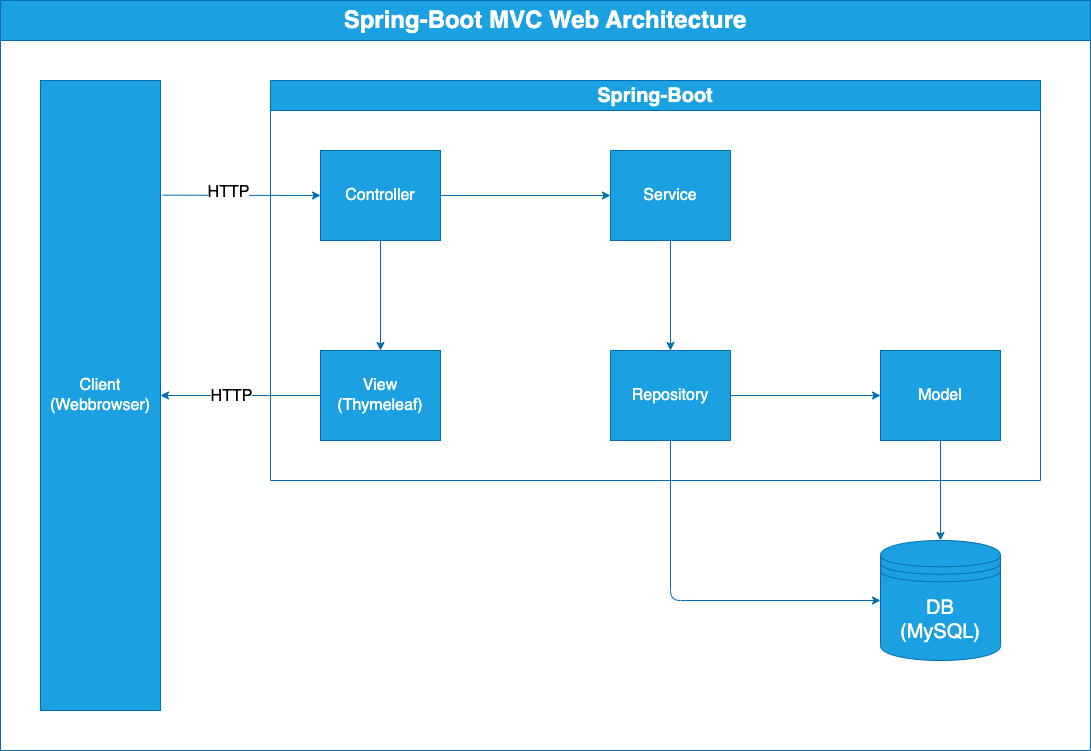
\includegraphics[scale=0.35]{Architektur.png}

    \subsection{Entity Relationship Diagramm}

    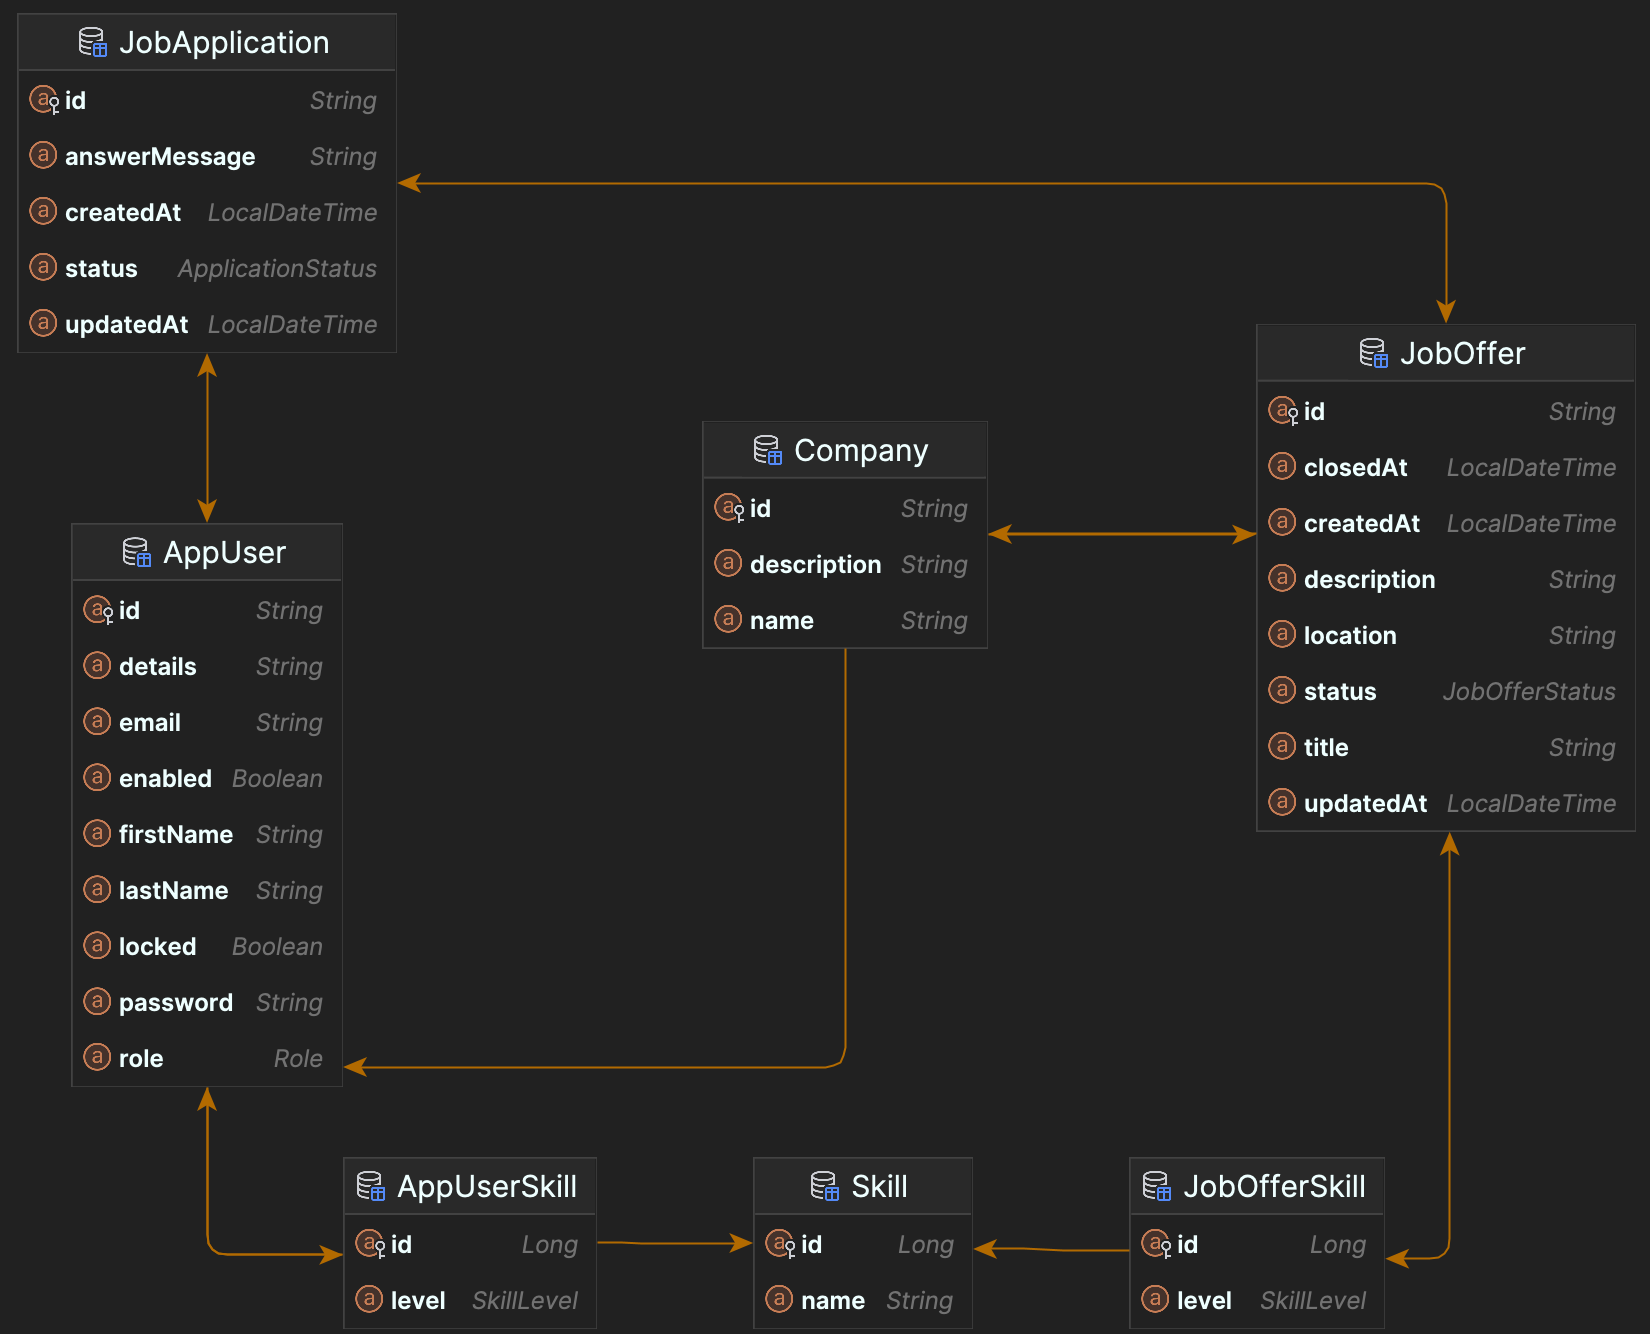
\includegraphics[scale=0.26]{erm2.png}

    \subsection{Sequenzdiagramme}

\end{document}